\chapter{Project and its goals}

Usability and user experience are major concerns in modern application development. With the proliferation of mobile devices and the explosion in the app market this has become an even bigger focus for developers as they strive to out compete others with polished and intuitive apps that explore new user interface paradigms suited to touch and smaller form factors.

Despite the simpler functionality that mobile apps tend to have compared to their desktop counterparts, creating an interface that is obvious to a newcomer to the application can still be a challenge. This is made worse by the relative recency and pace of evolution of mobile devices meaning that UI conventions are still in flux, and the limited screen real estate available on many devices forces developers to minimise space taken up by non-content.

\section{The Current Situation}

Testing the usability of an application’s interface is also one of the time consuming and resource intensive part of the testing process. Most other aspects of testing in application development, such as unit tests, integration tests, and even coverage tests for the user interface can easily be automated and run without any interaction from a human, since they are testing the correctness of the code in the application. Existing solutions for UI testing are aimed toward coverage testing - the test stresses the interface of the application by following a predefined model of interaction, or randomly taps areas of the UI for a period of time looking for unexpected ways to crash the application. On the android platform, a number of existing tools can be used to accomplish this, for example the Robotium \cite{robotium} framework, and monkey and monkeyrunner \cite{monkeyrunner} applications that ship with the Android developer tools. Usability testing on the other hand is not so simple, precisely because it is testing how a human reacts to the application compared to what is expected by the application’s developer.

\subsection{Traditional Usability testing}

Traditionally, usability testing is done by recruiting participants who are unfamiliar with the application being tested and chosen to cover the intended target audience as widely as possible. It usually takes place in a controlled setting designed to mimic, say, an office or living room, and the participant told to think aloud while trying to accomplish tasks given to them, based on work by K. A. Ericsson and H. A. Simon\cite{ericsson1980verbal}. This gives information about how the interface matches the participant’s thinking, and highlights areas that need improvement.

Since it it has such an overhead to set up and perform, individual hobbyist developers or even small companies with limited resources might shy away from performing usability testing. Even if it is done, it might not be done as regularly as might be optimal to catch design faults early in the process.

\section{A Search For a Better Way}

Modern software development is moving to a more iterative process with a “release early, release often” attitude. This trend is particularly visible in the mobile space, where the major platforms’ app stores provide an integrated and efficient delivery mechanism for updates. Combined with modern analytics packages and other user feedback mechanisms such as support emails and reviews this gives developers an opportunity to test their applications’ interface and gradually refine the user experience after release.

\subsection{Crowdsourcing}

Crowdsourcing has shown to be an effective way of performing repetitive tasks that aren't suitable for computers to perform - i.e. which need to be done by a human. It works by getting many people to perform a small amount of work, the results of which can be combined to form something useful. Perhaps some of the best known examples of applications employing crowdsourcing were created by Luis Von Ahn at Carnegie Mellon University, and include the ESP Game, where participants collaborate over the internet to assign machine readable tags to images, to help search results, reCAPTCHA, which leverages the popular “captcha” method of preventing automated bots from completing web forms to digitize books, and most recently Duolingo, a service which aims to teach people new languages while translating web pages.

Indeed when using analytics in an application this already seems like a form of crowdsourcing - the entire userbase of the application is potentially involved in the application’s improvement. However while analytics can be useful they lack the structured testing that is present with traditional user testing, and it can be difficult to interpret the data produced. UI usage is usually measured in the form of “events” that are triggered when a user performs an action in the application. For example in a music application, whenever the user presses a play button an event is sent to a remote server, and the developer can view statistics showing the number of people who pressed that button in a single day. By incorporating these events throughout the application, the developer can get a good idea of which parts of the application are heavily used, and what functionality is exerted more rarely. The obvious limitation of this approach is that it is difficult to discern the intent of the user; in most scenarios, the developer cannot distinguish between functionality that is not used because users have no desire to use it, and functionality that is not used because it is not obvious, or has poor usability. The exceptions here are use cases that have a specific workflow, for example a signup form or purchase, where events can be placed at each point of the process and the dropout rate at each stage can be measured.

\subsection{Gamification}

In the crowdsourcing examples given earlier, the ESP game and Duolingo have one thing in common - a way to keep people engaged so they continue using the application. The latter one does this by providing a useful service to the user, and the former by turning the experience into a game.

The process of integrating game oriented features into a non-gaming environment is known as Gamification, a concept that took off in mainstream computing around 2010 \cite{gamification-trends}. It commonly involves adding rewards such as points other forms of recognition for completing tasks or challenges within the environment.

It is possible that by incorporating ideas from crowdsourcing and gamification, and the techniques already used in mobile analytics, that a system can be created that provides useful feedback about the usability of a mobile application while having less cost and time overheads than traditional usability testing.

\section{Project Goals}

The aim of this project will be to investigate and implement a solution which can complement or even replace traditional usability testing during the development of a mobile application. It should allow the developer to test the application with users and obtain useful feedback about which parts of the user interface are easy to use, and which parts users find confusing or difficult.

\chapter{Design}

For the initial implementation, a single Android app was chosen to test. Despite this, the library should be generic enough to easily integrate into any Android application.

There are two core problems to solve. One is finding the best way to capture enough data from many users' interactions with the application and present it in a way that will highlight issues in the user interface. The second is keeping the participants engaged long enough to complete the testing, while using still the application in a natural way.

Due to the crowdsourced nature of the system, and the fact that no member of the development team will be present during the testing, the ``think aloud'' aspect of traditional testing will be missing. It would, of course, be possible to record the subject speaking as they navigate the application, but it would not be feasible to collect and aggregate that data automatically from many participants. Otherwise, the system will incorporate the same ideas as traditional usability testing.

\section{User Facing Design}

On starting the testing, the user is shown a screen explaining how the testing will work. They are then presented with a scenario/task for them to complete. On completion of the task, they will be either given a successive task, or a screen thanking them for participating. The developer will be able group a related series of tasks in a sequence that will be completed all at once.

To keep the participants engaged and to encourage them to continue with the testing, a gaming element is incorporated. The exact form this takes has evolved as the project has progressed (and may still change further!). In early iterations, an overlay would show how long the user is taking to complete the task (\emph{Figure \ref{fig:initial-overlay}}) and on completion of the task they would be assigned a number of points relative to how quickly they did it. There were a couple of concerns with this. Firstly, that showing the user how long they are taking and encouraging them to complete the task as quickly as possible would result in behaviour that does not match real world usage. Secondly, during trials of the prototypes, participants did not see any reason to gain more points since they were not used for anything, and weren't ranked e.g. against any other user.

\begin{figure}[ht!]
  \centering
  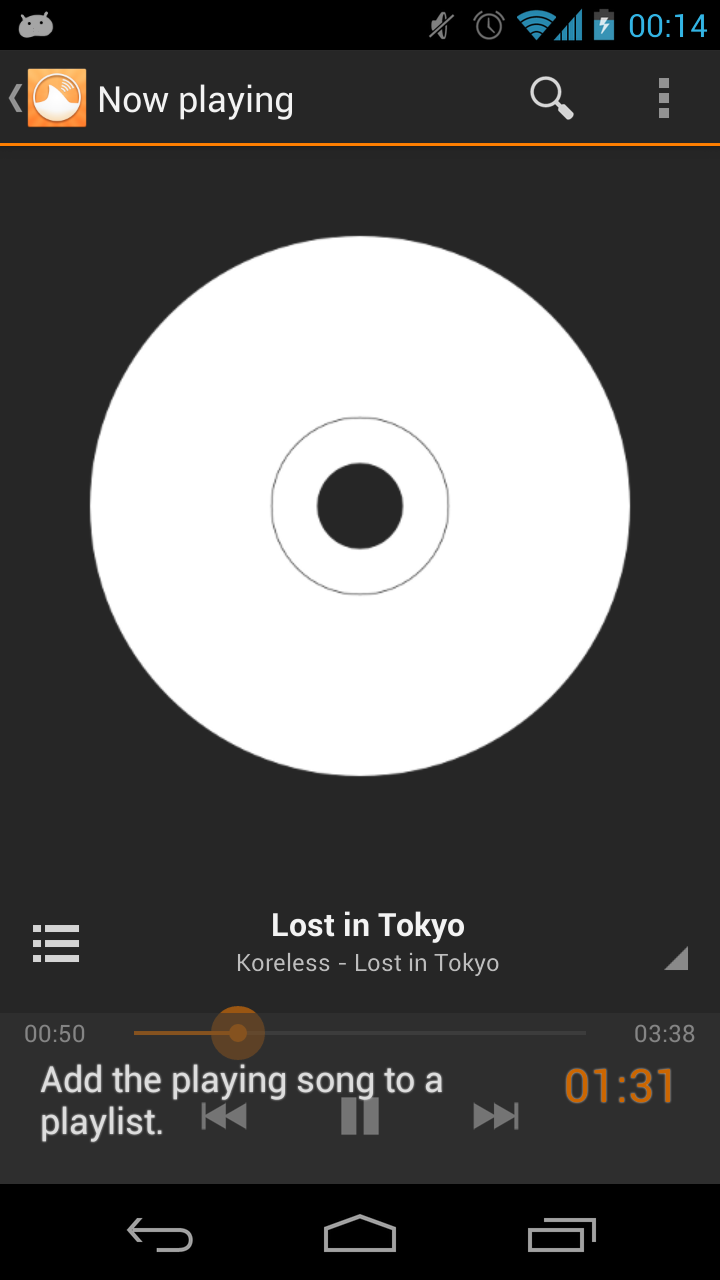
\includegraphics[width=0.5\textwidth]{images/time-taken}
  \caption{The task overlay in early iterations of the project.}
  \label{fig:initial-overlay}
\end{figure}

In the current iteration, the thank you screen will also show the user's ``tester rank'', which will depend on the amount of testing that they have completed compared with the number of tasks/sequences of tasks that are available within the application. This ranking will encourage the user to continue participating in the testing, and also allows for rewards (such as unlocking easter eggs or additional features within the app) if the developer wishes to include them.

The overlay that appears while performing a task is also being refined as early iterations, although being semi-transparent, still could obscure app content more than was desired.

\subsection{Abandoning Tasks}

It's likely that for some tasks, a participant might get stuck, and not be able to complete it. In these cases it seems unfair to penalise them, since the interface could be too unintuitive or confusing. Worse, this is usually the case where the developer could benefit most from the feedback, and if the participant were penalised it could discourage them from continuing with the testing. To combat this, as part of the overlay that appears while performing a task a button will allow the participant to abandon the current task at any point. If they do this, they will be presented with a form to provide written feedback about why they could not complete the task. Their ranking will still improve, since they have given useful feedback to the developer.

\section{Developer feedback}

For each task, the developer will be able to see aggregate data gathered from all participants. This will include, for example, the average time taken, the navigation path that participants took and other relevant data. For participants that abandoned the task, it will be possible to read any feedback that they provided.

\chapter{Implementation}

To allow easy integration into any Android app, the library will be implemented as an Android Library Project \cite{android-library}. It also needs to be easy to remove/disable if the developer does not want the testing functionality present for the released version.

\section{Integrating the Library}

In the current implementation, the developer creates two json files which are included in the application's \verb+assets/+ directory. All interaction with the library in performed using the static \verb/Gamify/ class. This allows for easy removal of the library, as the developer can just find all references to this class within the main application code and remove them. Since most Android developers use \emph{Proguard} while compiling release versions, a rule could be integrated to automatically strip the function calls out.

\begin{minted}{text}
  -assumenosideeffects class com.example.Gamify {
    <methods>;
  } 
\end{minted}

The library can also be disabled by passing \verb|false| when initialising. The initialisation is done by calling \verb|init| in either the \verb|Application| or initial \verb|Activity|'s \verb|onCreate| method, passing the two aforementioned json files.

\begin{minted}{java}
  Gamify.init(this /* Context */, true /* Enabled */,
      "challenges.json", "sequences.json");
\end{minted}

The ``challenges.json'' and ``sequences.json'' files define the tasks and challenges that will be used in testing, identified by ids. To start a sequence, the developer can simply call a single method, specifying the ID of the sequence to be started.

\begin{minted}{java}
  Gamify.startSequence("sequenceid");
\end{minted}

Triggering points that will complete tasks are achieved with another method call, for example if one task was completed by playing a song in the app, then the corresponding code might look like:

\begin{minted}{java}
  public void playSong(Song song) {
    Gamify.completeChallenge("playsong");
    
    //... Code to play the song
  }
\end{minted}

If the ``playsong'' task is the current task, then it will be completed, otherwise the method call will be ignored.

Beyond this, in each \verb|Activity|'s \verb|onResume| and \verb|onPause| methods, the library must be notified.

\begin{minted}{java}
  @Override
  protected void onResume() {
     super.onResume();

     Gamify.onActivityResume(this);
  }
  
  @Override
  protected void onPause() {
     super.onPause();

     Gamify.onActivityPause(this);
  }
\end{minted}

This is so user interaction can be tracked, and the library's overlays can be shown above the foreground activity. Since applications are usually designed so that all activities inherit from a single base activity, this does not add much extra overhead for the developer.

\section{Viewing the Data}

A companion application will run on a server and receive results from participants. This can be a simple web app that receives data sent by the Android app, validates it, and stores it in a database. A separate web application will retrieve the results from the database an display them to the developer.

These parts are currently mostly unimplemented, and will the be focus of the next few weeks of development.

\chapter{Timeline}

\section{What's Done}

\begin{itemize}
\item
Design and initial implementation of the library so that it can be included in any application.
\item
Integration of the library with a sample application.
\item
Testing with some users to gather feedback about the initial implementation. Aspects of how the game worked were changed and UI improvements were incorporated.
\item
Upload of test data to a remote server.
\end{itemize}

\section{Next Steps}

\subsection{Next Two Weeks}
\begin{itemize}
\item
Finish implementation of the library.
\item
Transform and display data gathered in a useful way.
\end{itemize}

\subsection{Before March}
\begin{itemize}
\item
Test with users, and evaluate data gathered.
\item
Implement library in an updated version of the test application and compare results.
\end{itemize}

\subsection{March - April}
\begin{itemize}
\item
Finish write-up.
\item
Perform any additional testing, perhaps trying to improve the data gathered.
\end{itemize}

